\documentclass[10pt]{article}
\usepackage[margin=0.8in]{geometry}

\usepackage[utf8]{inputenc}
\usepackage[T1]{fontenc}
\usepackage{amsmath}
\usepackage{amsfonts}
\usepackage{amssymb}
\usepackage[version=4]{mhchem}
\usepackage{stmaryrd}
\usepackage{graphicx}
\usepackage[export]{adjustbox}
\usepackage{bbold}
\usepackage{fixltx2e}
\usepackage{caption}
\usepackage{mathtools}
\usepackage{amsfonts} %% <- also included by amssymb
\DeclareMathSymbol{-}{\mathbin}{AMSa}{"39}
\usepackage[parfill]{parskip}
\usepackage{float}
\usepackage{url}
\usepackage{hyperref}

\usepackage[framemethod=TikZ]{mdframed}
\colorlet{shadecolor}{orange!15}
\usepackage{xcolor}
\usepackage{amsthm}
\usepackage{framed}





\begin{document}

\title{Lecture 6-8:  Denavit–Hartenberg Convention}
\date{Sep. 05, 2023 \quad Sep. 7, 2023 \quad Sep. 12, 2023 }
\author{Wanxin Jin}
\maketitle



A robot arm is a kinematic chain of rigid bodies (links) connected by actuated joints. One end of the kinematic chain is mounted to a base and the other end to an end-effector (gripper, tool). Joints have two typical types: revolute and prismatic, as  in Fig. \ref{c1.fig.joints-types}.  
The posture of a manipulator is described by a number of degrees of freedom (DOFs). Each DOF is typically associated with a joint variable. Manipulator (forward/direct) kinematics is to derive the relationship between joint motion and the motion of the end-effector.













\begin{figure}[h]
    \centering
   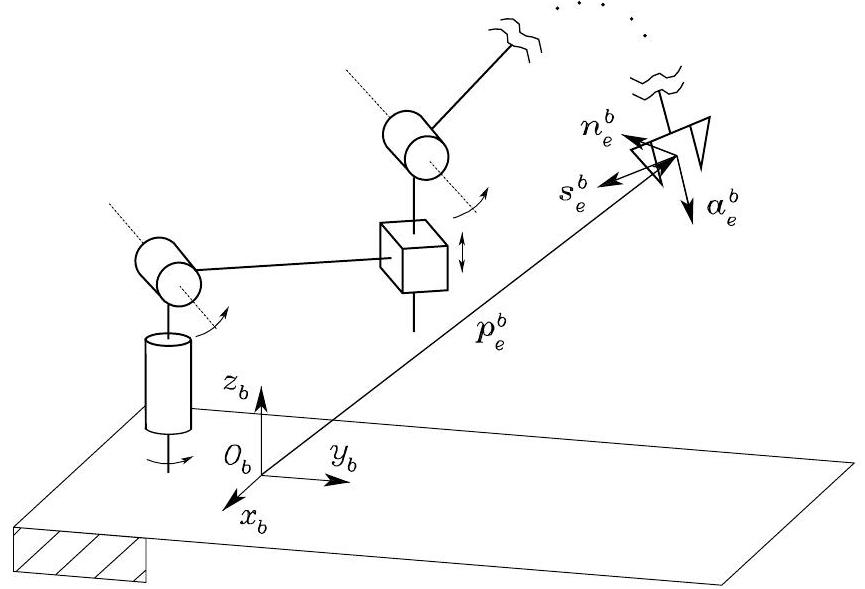
\includegraphics[max width=0.4\textwidth]{./kinematics/end-effector_frame}
    \caption{Description of the position and orientation of the end-effector frame}
    \label{c1.fig.joints-types}
\end{figure}

With respect to a base frame $O_{b}-x_{b} y_{b} z_{b}$, the  kinematics  is expressed by the homogeneous transformation 

$$
\boldsymbol{T}_{e}^{b}(\boldsymbol{q})=\left[\begin{array}{cccc}
\boldsymbol{n}_{e}^{b}(\boldsymbol{q}) & \boldsymbol{s}_{e}^{b}(\boldsymbol{q}) & \boldsymbol{a}_{e}^{b}(\boldsymbol{q}) & \boldsymbol{p}_{e}^{b}(\boldsymbol{q}) \\
0 & 0 & 0 & 1
\end{array}\right]
$$

where $\boldsymbol{q}$ is the $(n \times 1)$ vector of joint variables, $\{\boldsymbol{n}_{e}, \boldsymbol{s}_{e}, \boldsymbol{a}_{e}\}$ are the unit vectors of a frame attached to the end-effector, and $\boldsymbol{p}_{e}$ is the position  of the origin of the end-effector frame.  If the end-effector is a gripper, the origin of the end-effector frame is located at the center of the gripper,  $\boldsymbol{a}_{e}$ is chosen in the approach direction to the object, $\boldsymbol{s}_{e}$ is chosen normal to $\boldsymbol{a}_{e}$ in the sliding plane of the jaws, and  $\boldsymbol{n}_{e}$ is chosen to complete the right-handed rule.


\section{General Rule}
A manipulator chain composes of $n+1$ links connected by $n$ joints, where Link 0 is conventionally fixed to the ground/base. Each joint variable provides a single DOF. Define a frame attached to each link, from Link 0 to Link $n$. Then, the  transformation of Frame $n$ with respect to Frame 0 is 

$$
    \boldsymbol{T}_{n}^{0}(\boldsymbol{q})=\boldsymbol{A}_{1}^{0}\left(q_{1}\right) \boldsymbol{A}_{2}^{1}\left(q_{2}\right) \ldots \boldsymbol{A}_{n}^{n-1}\left(q_{n}\right) .
    $$

Computation is recursive by simple products of the homogeneous transformation matrices $\boldsymbol{A}_{i}^{i-1}\left(q_{i}\right)$ (for $\left.i=1, \ldots, n\right)$, each of which is a function of a single joint variable.
The kinematics describing the pose of the end-effector frame with respect to the base frame can be obtained as

$$
\boldsymbol{T}_{e}^{b}(\boldsymbol{q})=\boldsymbol{T}_{0}^{b} \boldsymbol{T}_{n}^{0}(\boldsymbol{q}) \boldsymbol{T}_{e}^{n}
$$

where $\boldsymbol{T}_{0}^{b}$ and $\boldsymbol{T}_{e}^{n}$ are two (typically) constant homogeneous transformations describing the position and orientation of Frame 0 with respect to the base frame, and of the end-effector frame with respect to Frame $n$, respectively.

\begin{figure}[h]
    \centering
   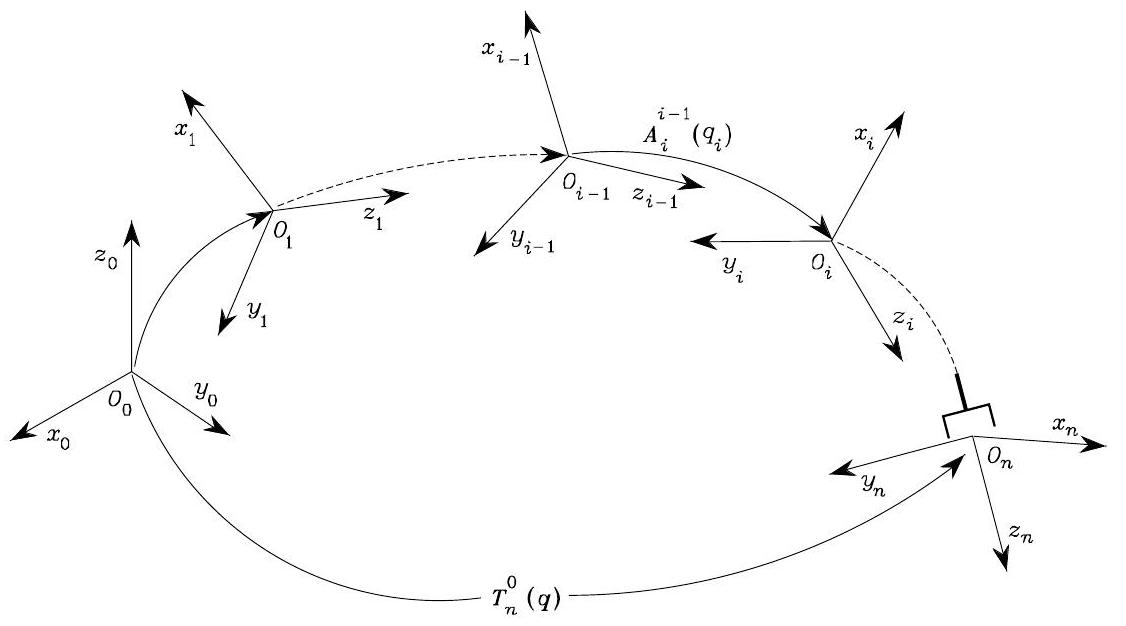
\includegraphics[max width=0.5\textwidth]{./kinematics/forward_kin}
    \caption{Kinematics of a robot manipulator}
    \label{c1.fig.joints-types}
\end{figure}

Then, the question is: how to select a frame for each link to compute $\boldsymbol{A}_{i}^{i-1}\left(q_{i}\right)$? (The answer is in the next section)







\section{Denavit-Hartenberg (DH) Convention}
 Denavit-Hartenberg (DH) Convention is to systematically and recursively define a frame to each link and obtain the transformation between two consecutive links.

\begin{figure}[H]
    \centering
   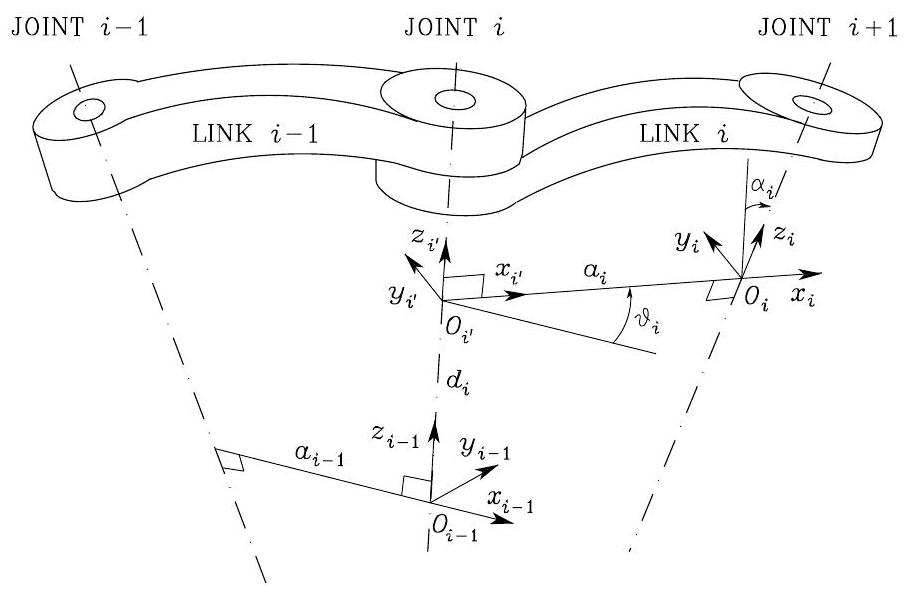
\includegraphics[max width=0.5\textwidth]{./kinematics/DH_convention}
    \caption{Denavit-Hartenberg convention and parameters for link Frame $i$}
    \label{c1.l2.dh}
\end{figure}







With reference to Fig. \ref{c1.l2.dh}, joint $i$ connects Link $i-1$ to Link $i$;   DH convention  sets the following rules to define link Frame $O_{i}-x_{i} y_{i} z_{i}$, given previous link Frame  $O_{i-1}-x_{i-1} y_{i-1} z_{i-1}$:

\begin{itemize}
  \item Choose axis $z_{i}$ along the joint $i+1$.

  \item Locate the origin $O_{i}$ at the intersection of axis $z_{i}$ with the common normal to axes $z_{i}$ and $z_{i-1}$ . Also, locate an intermediate point $O_{i^{\prime}}$ at the intersection of the common normal with axis $z_{i-1}$.

  \item Choose axis $x_{i}$ along the common normal to axes $z_{i-1}$ and $z_{i}$ with direction from Joint $i$ to Joint $i+1$.

  \item Choose axis $y_{i}$ to complete a right-handed frame.
\end{itemize}





\noindent
Once the link frames are established, the position and orientation of   link Frame $O_{i}-x_{i} y_{i} z_{i}$ with respect to link Frame  $O_{i-1}-x_{i-1} y_{i-1} z_{i-1}$ have been determined by the following four parameters:


    - $a_{i}$ distance between $O_{i}$ and $O_{i^{\prime}}$ --- constant and depend only on the geometry of links\\
     - $\alpha_{i}$ angle between axes $z_{i-1}$ and $z_{i}$ about axis $x_{i}$  --- constant and depend only on the geometry of links\\
     - $d_{i}$ distance of between $O_{i-1}$ and $O_{i^{\prime}}$ along $z_{i-1}$ ---  variable if Joint $i$ is prismatic,  otherwise constant\\
    - $\vartheta_{i}$ angle between axes $x_{i-1}$ and $x_{i}$ about axis $z_{i-1}$ ---  variable 

\noindent
To  compute $\boldsymbol{A}_{i}^{i-1}\left(q_{i}\right)$, we go the following steps. First,  translate the   Frame  $O_{i-1}-x_{i-1} y_{i-1} z_{i-1}$ by $d_{i}$ along axis $z_{i-1}$ and rotate it by $\vartheta_{i}$ about axis $z_{i-1}$; this leads to the following transformation of the intermediate Frame $i^{\prime}$ 

$$
\boldsymbol{A}_{i^{\prime}}^{i-1}=\left[\begin{array}{cccc}
c_{\vartheta_{i}} & -s_{\vartheta_{i}} & 0 & 0 \\
s_{\vartheta_{i}} & c_{\vartheta_{i}} & 0 & 0 \\
0 & 0 & 1 & d_{i} \\
0 & 0 & 0 & 1
\end{array}\right]
$$

Second,  translate the  intermediate Frame $i^{\prime}$ by $a_{i}$ along axis $x_{i^{\prime}}$ and rotate it by $\alpha_{i}$ about axis $x_{i^{\prime}}$; this  leads to the following transformation and Frame $O_{i}-x_{i} y_{i} z_{i}$. 

$$
\boldsymbol{A}_{i}^{i^{\prime}}=\left[\begin{array}{cccc}
1 & 0 & 0 & a_{i} \\
0 & c_{\alpha_{i}} & -s_{\alpha_{i}} & 0 \\
0 & s_{\alpha_{i}} & c_{\alpha_{i}} & 0 \\
0 & 0 & 0 & 1
\end{array}\right]
$$

Thus, the total transformation is obtained by \emph{postmultiplication rule}



$$
\boldsymbol{A}_{i}^{i-1}\left(q_{i}\right)=\boldsymbol{A}_{i^{\prime}}^{i-1} \boldsymbol{A}_{i}^{i^{\prime}}=\left[\begin{array}{cccc}
c_{\vartheta_{i}} & -s_{\vartheta_{i}} c_{\alpha_{i}} & s_{\vartheta_{i}} s_{\alpha_{i}} & a_{i} c_{\vartheta_{i}} \\
s_{\vartheta_{i}} & c_{\vartheta_{i}} c_{\alpha_{i}} & -c_{\vartheta_{i}} s_{\alpha_{i}} & a_{i} s_{\vartheta_{i}} \\
0 & s_{\alpha_{i}} & c_{\alpha_{i}} & d_{i} \\
0 & 0 & 0 & 1
\end{array}\right]
$$




The DH convention gives a nonunique definition of the link frame in the following cases. (1) For Frame 0, only the direction of axis $z_{0}$ is specified; then $O_{0}$ and $x_{0}$ can be arbitrarily chosen. (2) For Frame $n$, since there is no Joint $n+1, z_{n}$ is not uniquely defined while $x_{n}$ has to be normal to axis $z_{n-1}$. Typically, Joint $n$ is revolute, and thus $z_{n}$ is to be aligned with the direction of $z_{n-1}$. (3) When two consecutive axes intersect, the direction of $x_{i}$ is arbitrary. and (4) When Joint $i$ is prismatic, the direction of $z_{i-1}$ is arbitrary. In all such cases, the principle of choosing frames is to simplify the procedure; for instance, the axes of consecutive frames can be made parallel.






\noindent
To summarize, we write the following Algorithm to use DH convention for a robot manipulator.

\begin{enumerate}
  \item Find and number each joint and  set the directions of axes $z_{0}, \ldots, z_{n-1}$

  \item Choose Frame   $O_{0}-x_{0} y_{0} z_{0}$. If possible,  choose $\{\boldsymbol{x}_{0}, \boldsymbol{y}_{0}, \boldsymbol{z}_{0}\}$ to coincide with the base frame.

\end{enumerate}

Execute steps from 3 for $i=1, \ldots, n-1$ :

\begin{enumerate}
  \setcounter{enumi}{2}
  \item Choose Frame   $O_{i}-x_{i} y_{i} z_{i}$ using the following rules. 
  First, choose $O_{i}$ at the intersection of $z_{i}$ with the common normal to  $z_{i-1}$ and $z_{i}$. If  $z_{i-1}$ and $z_{i}$ are parallel and Joint $i$ is revolute, choose $O_{i}$ so that $d_{i}=0$; if Joint $i$ is prismatic, choose $O_{i}$ at as a mechanical limit. Second, choose axis $x_{i}$ along the common normal to axes $z_{i-1}$ and $z_{i}$ with direction from Joint $i$ to Joint $i+1$, Third, choose axis $y_{i}$ so as to obtain a right-handed frame.

\end{enumerate}

To complete:

\begin{enumerate}
  \setcounter{enumi}{3}
  \item Choose Frame $O_{n}-x_{n} y_{n} z_{n}$; if Joint $n$ is revolute, then align $z_{n}$ with $z_{n-1}$, otherwise, if Joint $n$ is prismatic, then choose $z_{n}$ arbitrarily. choose axis $x_{n}$ along the common normal to axes $z_{n-1}$ and $z_{n}$.

  \item For $i=1, \ldots, n$, establish the DH parameter table $a_{i}, d_{i}, \alpha_{i}, \vartheta_{i}$,
  compute the homogeneous transformation matrices $\boldsymbol{A}_{i}^{i-1}\left(q_{i}\right)$, and compute the homogeneous transformation $\boldsymbol{T}_{n}^{0}(\boldsymbol{q})=\boldsymbol{A}_{1}^{0} \ldots \boldsymbol{A}_{n}^{n-1}$ that yields the pose of Frame $n$ with respect to Frame 0 .
  
  \item Given $\boldsymbol{T}_{0}^{b}$ and $\boldsymbol{T}_{e}^{n}$, compute the  kinematics function as $\boldsymbol{T}_{e}^{b}(\boldsymbol{q})=$ $\boldsymbol{T}_{0}^{b} \boldsymbol{T}_{n}^{0} \boldsymbol{T}_{e}^{n}$.

\end{enumerate}



\section{Kinematics of Typical Manipulators}






\subsection{Three-link Planar Arm}
\begin{figure}[H]
    \centering
   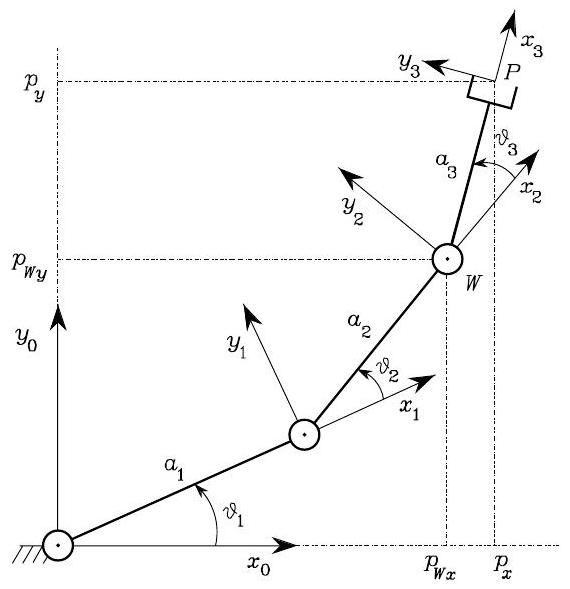
\includegraphics[max width=0.25\textwidth]{./kinematics/3link_arm}
    \label{c1.l2.three-link-robot-arm}
\end{figure}




\begin{table}[h]
\begin{center}
\begin{tabular}{ccccc}
\hline
Link & $a_{i}$ & $\alpha_{i}$ & $d_{i}$ & $\vartheta_{i}$ \\
\hline
1 & $a_{1}$ & 0 & 0 & $\vartheta_{1}$ \\
2 & $a_{2}$ & 0 & 0 & $\vartheta_{2}$ \\
3 & $a_{3}$ & 0 & 0 & $\vartheta_{3}$ \\
\hline
\end{tabular}
\label{c1.l2.table.three-link-dh}
\end{center}
\end{table}

\noindent
$$
    \boldsymbol{T}_{3}^{0}(\boldsymbol{q})=\boldsymbol{A}_{1}^{0} \boldsymbol{A}_{2}^{1} \boldsymbol{A}_{3}^{2}=\left[\begin{array}{cccc}
c_{123} & -s_{123} & 0 & a_{1} c_{1}+a_{2} c_{12}+a_{3} c_{123} \\
s_{123} & c_{123} & 0 & a_{1} s_{1}+a_{2} s_{12}+a_{3} s_{123} \\
0 & 0 & 1 & 0 \\
0 & 0 & 0 & 1
\end{array}\right]
$$





\subsection{Spherical Arm}
\begin{figure}[H]
    \centering
   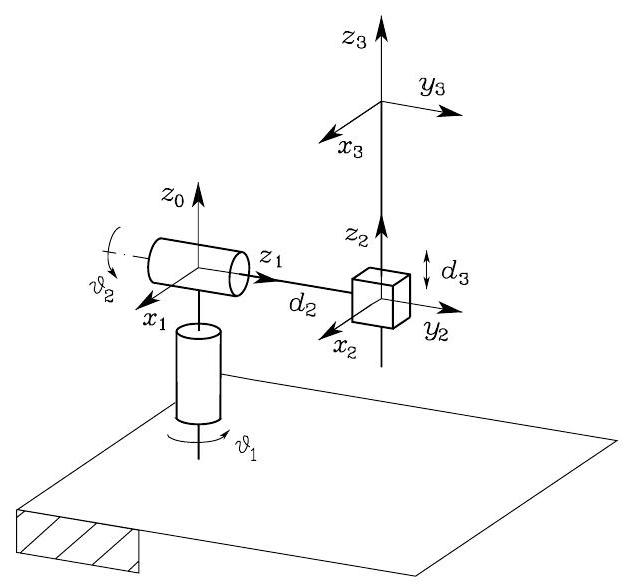
\includegraphics[max width=0.3\textwidth]{./kinematics/spherical_arm}
    \label{c1.l2.fig.spherical-arm}
\end{figure}




\begin{table}[h]
\begin{center}
\begin{tabular}{ccccc}
\hline
Link & $a_{i}$ & $\alpha_{i}$ & $d_{i}$ & $\vartheta_{i}$ \\
\hline
1 & 0 & $-\pi / 2$ & 0 & $\vartheta_{1}$ \\
2 & 0 & $\pi / 2$ & $d_{2}$ & $\vartheta_{2}$ \\
3 & 0 & 0 & $d_{3}$ & 0 \\
\hline
\end{tabular}
\end{center}
\end{table}


$$
\boldsymbol{T}_{3}^{0}(\boldsymbol{q})=\boldsymbol{A}_{1}^{0} \boldsymbol{A}_{2}^{1} \boldsymbol{A}_{3}^{2}=\left[\begin{array}{cccc}
c_{1} c_{2} & -s_{1} & c_{1} s_{2} & c_{1} s_{2} d_{3}-s_{1} d_{2} \\
s_{1} c_{2} & c_{1} & s_{1} s_{2} & s_{1} s_{2} d_{3}+c_{1} d_{2} \\
-s_{2} & 0 & c_{2} & c_{2} d_{3} \\
0 & 0 & 0 & 1
\end{array}\right]
$$

\subsection{Anthropomorphic Arm}

\begin{figure}[H]
    \centering
   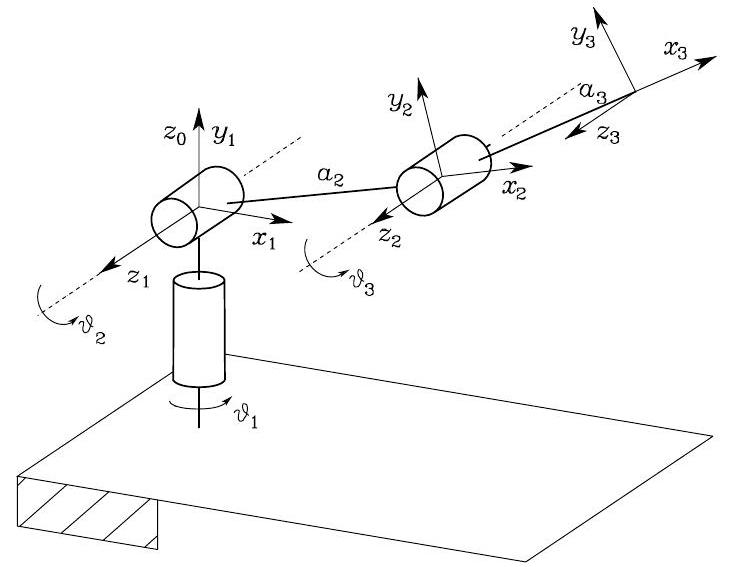
\includegraphics[max width=0.3\textwidth]{./kinematics/anthropomorphic_arm}
\end{figure}

\begin{table}[h]
    \centering
\begin{tabular}{ccccc}
\hline
Link & $a_{i}$ & $\alpha_{i}$ & $d_{i}$ & $\vartheta_{i}$ \\
\hline
1 & 0 & $\pi / 2$ & 0 & $\vartheta_{1}$ \\
2 & $a_{2}$ & 0 & 0 & $\vartheta_{2}$ \\
3 & $a_{3}$ & 0 & 0 & $\vartheta_{3}$ \\
\hline
\end{tabular}
    \label{c1.l2.table.anthropomorphic}
\end{table}



$$
\boldsymbol{T}_{3}^{0}(\boldsymbol{q})=\boldsymbol{A}_{1}^{0} \boldsymbol{A}_{2}^{1} \boldsymbol{A}_{3}^{2}=\left[\begin{array}{cccc}
c_{1} c_{23} & -c_{1} s_{23} & s_{1} & c_{1}\left(a_{2} c_{2}+a_{3} c_{23}\right) \\
s_{1} c_{23} & -s_{1} s_{23} & -c_{1} & s_{1}\left(a_{2} c_{2}+a_{3} c_{23}\right) \\
s_{23} & c_{23} & 0 & a_{2} s_{2}+a_{3} s_{23} \\
0 & 0 & 0 & 1
\end{array}\right]
$$



\subsection{Spherical Wrist}

\begin{figure}[H]
    \centering
   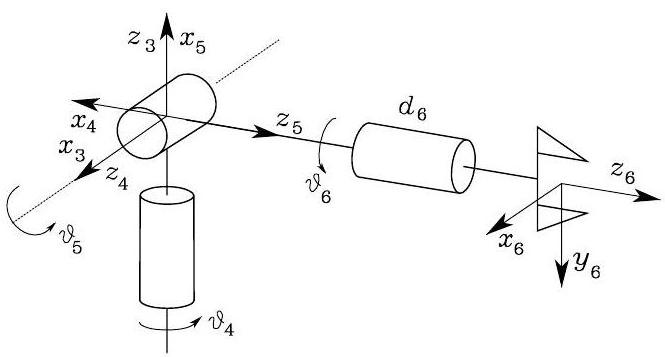
\includegraphics[max width=0.35\textwidth]{./kinematics/spherical_wrist}
\end{figure}



\begin{table}[h]
    \centering
\begin{tabular}{ccccc}
\hline
${\text { Link }}$ & $a_{i}$ & $\alpha_{i}$ & $d_{i}$ & $\vartheta$ \\
\hline
4 & 0 & $-\pi / 2$ & 0 & $\vartheta$ \\
5 & 0 & $\pi / 2$ & 0 & $\vartheta_{5}$ \\
6 & 0 & 0 & $d_{6}$ & $\vartheta_{6}$ \\
\hline
\end{tabular}
\end{table}





\noindent
Direct kinematics 
$$
\boldsymbol{T}_{6}^{3}(\boldsymbol{q})=\boldsymbol{A}_{4}^{3} \boldsymbol{A}_{5}^{4} \boldsymbol{A}_{6}^{5}=\left[\begin{array}{cccc}
c_{4} c_{5} c_{6}-s_{4} s_{6} & -c_{4} c_{5} s_{6}-s_{4} c_{6} & c_{4} s_{5} & c_{4} s_{5} d_{6} \\
s_{4} c_{5} c_{6}+c_{4} s_{6} & -s_{4} c_{5} s_{6}+c_{4} c_{6} & s_{4} s_{5} & s_{4} s_{5} d_{6} \\
-s_{5} c_{6} & s_{5} s_{6} & c_{5} & c_{5} d_{6} \\
0 & 0 & 0 & 1
\end{array}\right]
$$


where $\boldsymbol{q}=\left[\begin{array}{lll}\vartheta_{4} & \vartheta_{5} & \vartheta_{6}\end{array}\right]^{T}$. 

\smallskip

\emph{Notice that $\boldsymbol{R}_{6}^{3}$ coincides with the rotation matrix of Euler angles previously derived, that is, $\vartheta_{4}, \vartheta_{5}, \vartheta_{6}$ constitute the set of $\mathrm{ZYZ}$ angles with respect to the reference frame $O_{3}-x_{3} y_{3} z_{3}$.
}

\subsection{Stanford Manipulator}










\begin{figure}[H]
    \centering
    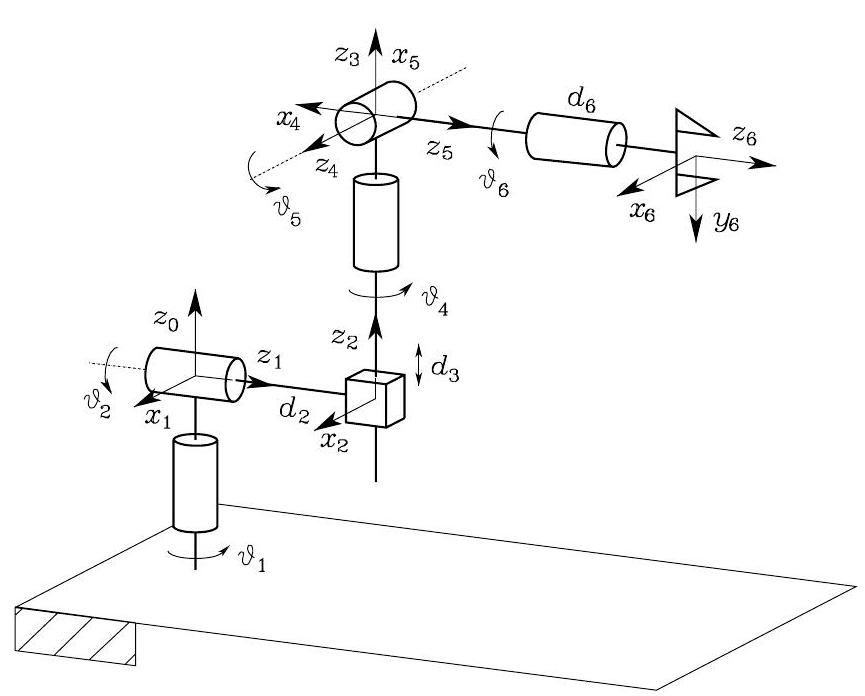
\includegraphics[max width=0.45\textwidth]{./kinematics/Stanford_manipulator}
    \label{c1.l2.fig.Stanford}
\end{figure}




$$
\boldsymbol{T}_{6}^{0}=\boldsymbol{T}_{3}^{0} \boldsymbol{T}_{6}^{3}=\left[\begin{array}{cccc}
\boldsymbol{n}^{0} & \boldsymbol{s}^{0} & \boldsymbol{a}^{0} & \boldsymbol{p}^{0} \\
0 & 0 & 0 & 1
\end{array}\right]
$$

\noindent
with

$$
\boldsymbol{p}_{6}^{0}=\left[\begin{array}{c}
c_{1} s_{2} d_{3}-s_{1} d_{2}+\left(c_{1}\left(c_{2} c_{4} s_{5}+s_{2} c_{5}\right)-s_{1} s_{4} s_{5}\right) d_{6} \\
s_{1} s_{2} d_{3}+c_{1} d_{2}+\left(s_{1}\left(c_{2} c_{4} s_{5}+s_{2} c_{5}\right)+c_{1} s_{4} s_{5}\right) d_{6} \\
c_{2} d_{3}+\left(-s_{2} c_{4} s_{5}+c_{2} c_{5}\right) d_{6}
\end{array}\right]
$$



$$
\begin{aligned}
& \boldsymbol{n}_{6}^{0}= {\left[\begin{array}{c}
c_{1}\left(c_{2}\left(c_{4} c_{5} c_{6}-s_{4} s_{6}\right)-s_{2} s_{5} c_{6}\right)-s_{1}\left(s_{4} c_{5} c_{6}+c_{4} s_{6}\right) \\
s_{1}\left(c_{2}\left(c_{4} c_{5} c_{6}-s_{4} s_{6}\right)-s_{2} s_{5} c_{6}\right)+c_{1}\left(s_{4} c_{5} c_{6}+c_{4} s_{6}\right) \\
-s_{2}\left(c_{4} c_{5} c_{6}-s_{4} s_{6}\right)-c_{2} s_{5} c_{6}
\end{array}\right] } \\
& \boldsymbol{s}_{6}^{0}=\left[\begin{array}{c}
c_{1}\left(-c_{2}\left(c_{4} c_{5} s_{6}+s_{4} c_{6}\right)+s_{2} s_{5} s_{6}\right)-s_{1}\left(-s_{4} c_{5} s_{6}+c_{4} c_{6}\right) \\
s_{1}\left(-c_{2}\left(c_{4} c_{5} s_{6}+s_{4} c_{6}\right)+s_{2} s_{5} s_{6}\right)+c_{1}\left(-s_{4} c_{5} s_{6}+c_{4} c_{6}\right) \\
s_{2}\left(c_{4} c_{5} s_{6}+s_{4} c_{6}\right)+c_{2} s_{5} s_{6}
\end{array}\right] \\
& \boldsymbol{a}_{6}^{0}=\left[\begin{array}{c}
c_{1}\left(c_{2} c_{4} s_{5}+s_{2} c_{5}\right)-s_{1} s_{4} s_{5} \\
s_{1}\left(c_{2} c_{4} s_{5}+s_{2} c_{5}\right)+c_{1} s_{4} s_{5} \\
-s_{2} c_{4} s_{5}+c_{2} c_{5}
\end{array}\right]
\end{aligned}
$$




\subsection{Anthropomorphic Arm with Spherical Wrist}


\begin{figure}[H]
    \centering
    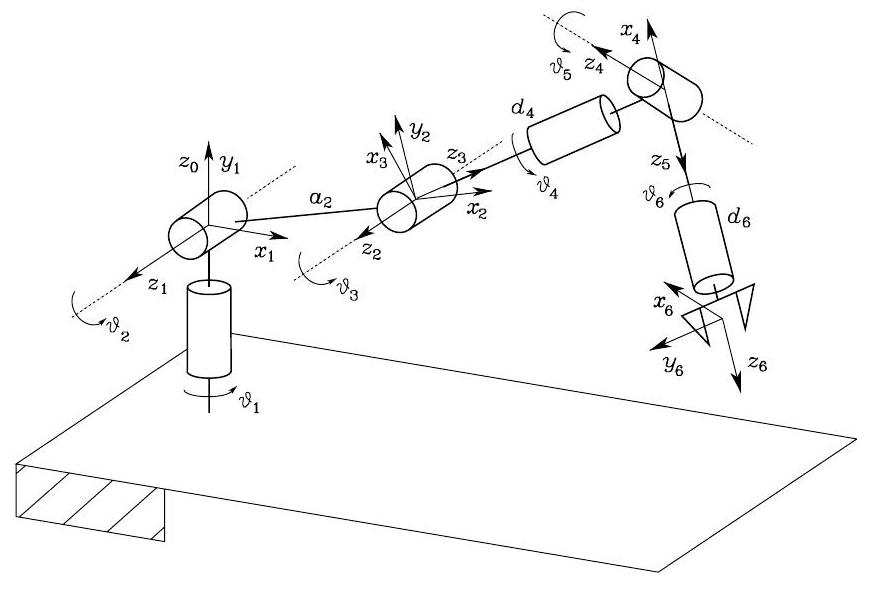
\includegraphics[max width=0.45\textwidth]{./kinematics/anthropomorphic_manipulator}
    \label{c1.l2.fig.anthropomorphic-wrist}
\end{figure}


\begin{table}[H]
    \centering
\begin{tabular}{ccccc}
\hline
Link & $a_{i}$ & $\alpha_{i}$ & $d_{i}$ & $\vartheta_{i}$ \\
\hline
1 & 0 & $\pi / 2$ & 0 & $\vartheta_{1}$ \\
2 & $a_{2}$ & 0 & 0 & $\vartheta_{2}$ \\
3 & 0 & $\pi / 2$ & 0 & $\vartheta_{3}$ \\
4 & 0 & $-\pi / 2$ & $d_{4}$ & $\vartheta_{4}$ \\
5 & 0 & $\pi / 2$ & 0 & $\vartheta_{5}$ \\
6 & 0 & 0 & $d_{6}$ & $\vartheta_{6}$ \\
\hline
\end{tabular}
\end{table}

\noindent
$$
\boldsymbol{T}_{6}^{0}=\left[\begin{array}{cccc}
\boldsymbol{n}^{0} & \boldsymbol{s}^{0} & \boldsymbol{a}^{0} & \boldsymbol{p}^{0} \\
0 & 0 & 0 & 1
\end{array}\right]
$$

with


$$
\begin{aligned}
\boldsymbol{p}_{6}^{0}=&\left[\begin{array}{c}
a_{2} c_{1} c_{2}+d_{4} c_{1} s_{23}+d_{6}\left(c_{1}\left(c_{23} c_{4} s_{5}+s_{23} c_{5}\right)+s_{1} s_{4} s_{5}\right) \\
a_{2} s_{1} c_{2}+d_{4} s_{1} s_{23}+d_{6}\left(s_{1}\left(c_{23} c_{4} s_{5}+s_{23} c_{5}\right)-c_{1} s_{4} s_{5}\right) \\
a_{2} s_{2}-d_{4} c_{23}+d_{6}\left(s_{23} c_{4} s_{5}-c_{23} c_{5}\right)
\end{array}\right]\\
\boldsymbol{n}_{6}^{0}= & {\left[\begin{array}{c}
c_{1}\left(c_{23}\left(c_{4} c_{5} c_{6}-s_{4} s_{6}\right)-s_{23} s_{5} c_{6}\right)+s_{1}\left(s_{4} c_{5} c_{6}+c_{4} s_{6}\right) \\
s_{1}\left(c_{23}\left(c_{4} c_{5} c_{6}-s_{4} s_{6}\right)-s_{23} s_{5} c_{6}\right)-c_{1}\left(s_{4} c_{5} c_{6}+c_{4} s_{6}\right) \\
s_{23}\left(c_{4} c_{5} c_{6}-s_{4} s_{6}\right)+c_{23} s_{5} c_{6}
\end{array}\right] } \\
\boldsymbol{s}_{6}^{0}= & {\left[\begin{array}{c}
c_{1}\left(-c_{23}\left(c_{4} c_{5} s_{6}+s_{4} c_{6}\right)+s_{23} s_{5} s_{6}\right)+s_{1}\left(-s_{4} c_{5} s_{6}+c_{4} c_{6}\right) \\
s_{1}\left(-c_{23}\left(c_{4} c_{5} s_{6}+s_{4} c_{6}\right)+s_{23} s_{5} s_{6}\right)-c_{1}\left(-s_{4} c_{5} s_{6}+c_{4} c_{6}\right) \\
-s_{23}\left(c_{4} c_{5} s_{6}+s_{4} c_{6}\right)-c_{23} s_{5} s_{6}
\end{array}\right] } \\
\boldsymbol{a}_{6}^{0}= & {\left[\begin{array}{c}
c_{1}\left(c_{23} c_{4} s_{5}+s_{23} c_{5}\right)+s_{1} s_{4} s_{5} \\
s_{1}\left(c_{23} c_{4} s_{5}+s_{23} c_{5}\right)-c_{1} s_{4} s_{5} \\
s_{23} c_{4} s_{5}-c_{23} c_{5}
\end{array}\right] }
\end{aligned}
$$









\section{Workspace}

The manipulator workspace is the space reached by the origin of the end-effector frame when the manipulator's joints tasks all allowable values. The workspace includes reachable workspace and dexterous workspace. The latter is the space that the origin of the end-effector frame can reach with different orientations, while the former is the space that the origin of the end-effector frame can reach with at least one orientation. 

For an $n$-DOF manipulator, the reachable workspace is the geometric locus of the points that can be achieved by considering the direct kinematics equation for the position part, i.e.,

$$
\boldsymbol{p}_{e}=\boldsymbol{p}_{e}(\boldsymbol{q}), \quad q_{i m} \leq q_{i} \leq q_{i M} \quad i=1, \ldots, n,
$$

where $q_{i m}\left(q_{i M}\right)$ denotes the minimum (maximum) limit at Joint $i$. The manipulator workspace (without end-effector) is reported in the data sheet given by the robot manufacturer in terms of a top view and a side view. 


In a manipulator, if actual mechanical parameters differ from the nominal value of  parameters in data sheet, a deviation arises between the actual position reached and the position computed via direct kinematics. Such a deviation is defined accuracy.  Accuracy attains typical values below one millimeter and depends on the structure as well as on manipulator dimensions. Another parameter that is usually listed in the performance data sheet of an industrial robot is repeatability which gives a measure of the manipulator's ability to return to a previously reached position. Repeatability depends not only on the mechanical structure but also on the transducers and controller; it is expressed in metric units and is typically smaller than accuracy. For instance, for a manipulator with a maximum reach of $1.5 \mathrm{~m}$, accuracy varies from 0.2 to $1 \mathrm{~mm}$ in the workspace, while repeatability varies from 0.02 to $0.2 \mathrm{~mm}$.


\section{Kinematic Redundancy}

A manipulator is termed kinematically redundant when it has a number of DOFs which is greater than the number of variables that are necessary to describe a given task. With reference to the above-defined spaces, a manipulator is intrinsically redundant when the dimension of the operational space is smaller than the dimension of the joint space $(m<n)$. Redundancy is, anyhow, a concept relative to the task assigned to the manipulator; a manipulator can be redundant with respect to a task and nonredundant with respect to another. Even in the case of $m=n$, a manipulator can be functionally redundant when only a number of $r$ components of operational space are of concern for the specific task, with $r<m$.

Consider again the three-DOF planar arm. If only the endeffector position (in the plane) is specified, that structure presents a functional redundancy $(n=m=3, r=2)$; this is lost when also the end-effector orientation in the plane is specified $(n=m=r=3)$. On the other hand, a four-DOF planar arm is intrinsically redundant $(n=4, m=3)$.
Yet, take the typical industrial robot with six DOFs; such manipulator is not intrinsically redundant $(n=m=6)$, but it can become functionally redundant with regard to the task to execute. Thus, for instance, in a lasercutting task a functional redundancy will occur since the end-effector rotation about the approach direction is irrelevant to completion of the task $(r=5)$.

At this point, a question should arise spontaneously: Why to intentionally utilize a redundant manipulator? The answer is to recognize that redundancy can provide the manipulator with dexterity and versatility in its motion. The typical example is constituted by the human arm that has seven DOFs: three in the shoulder, one in the elbow and three in the wrist, without considering the DOFs in the fingers. This manipulator is intrinsically redundant; in fact, if the base and the hand position and orientation are both fixed - requiring six DOFs - the elbow can be moved, thanks to the additional available DOF Then, for instance, it is possible to avoid obstacles in the workspace. Further, if a joint of a redundant manipulator reaches its mechanical limit, there might be other joints that allow execution of the prescribed end-effector motion.






\section{Modified DH parameters \& Panda Robot Arm}




\begin{figure}[H]
    \centering
    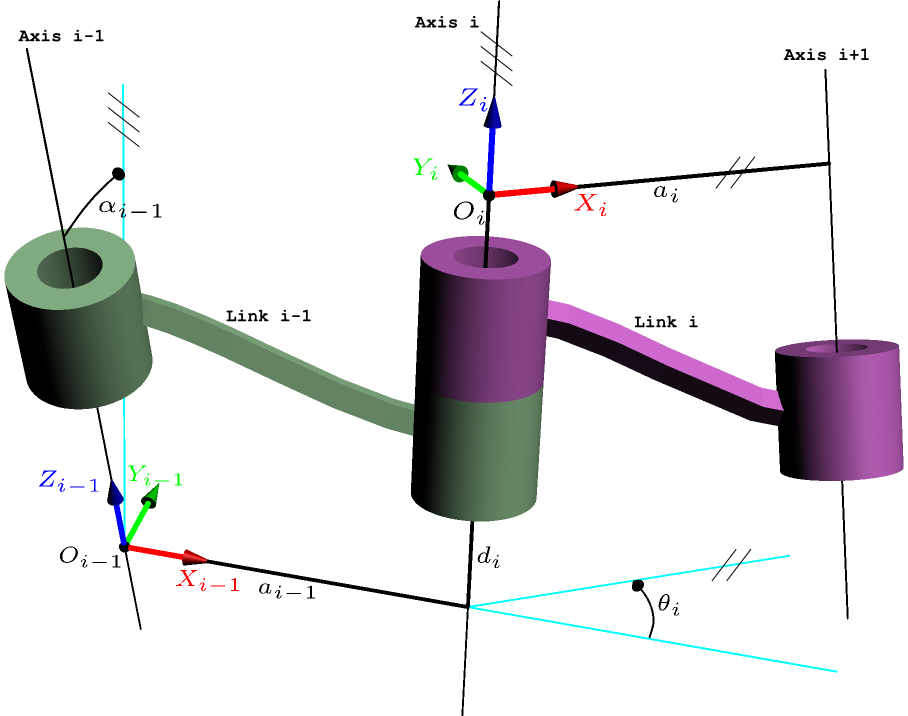
\includegraphics[max width=0.6\textwidth]{kinematics/DHParameter.png}
    \caption{Modified DH parameters (or called Craig's convention). Image from Wiki}
\end{figure}


Some books use modified (proximal) DH parameters [John J. Craig, Introduction to Robotics: Mechanics and Control (3rd Edition)]. The difference between the classic (distal) DH parameters and the modified DH parameters are the locations of the coordinates system attachment to the links and the order of the performed transformations.


Compared with the classic DH parameters, the coordinates of frame, $O_{i-1}$, is put on Joint $i-1$, not the Joint $i$ in classic DH convention;the coordinates of frame, $O_{i}$, is put on Joint $i$, not the Joint $i+1$ in classic DH convention. Another difference is that according to the modified convention, the transform matrix is given by the following order of operations:

$$
^{i-1}T_i=\text{Rot}_{x_{i-1}}(\alpha_{i-1})\text{Trans}_{x_{i-1}}(a_{i-1})\text{Rot}_{z_{i}}(\theta_{i})\text{Trans}_{z_{i}}(d_{i})
$$

One example of using the above modified DH convention is Franka-Emika Panda robot arm, an increasingly popular robot for research and teaching.  It has 7 joints which make it a redundant robot, that is, it has more joints than it needs to achieve an arbitrary position and orientation in the Cartesian workspace. 


The DH parameter defined for Panda Robot arm is as follows: \url{https://frankaemika.github.io/docs/control_parameters.html}. Please find a great  tutorial (using Python) about Panda Arm's forward kinematics at 


\href{https://github.com/jhavl/dkt}{https://github.com/jhavl/dkt}



\begin{figure}[H]
    \centering
    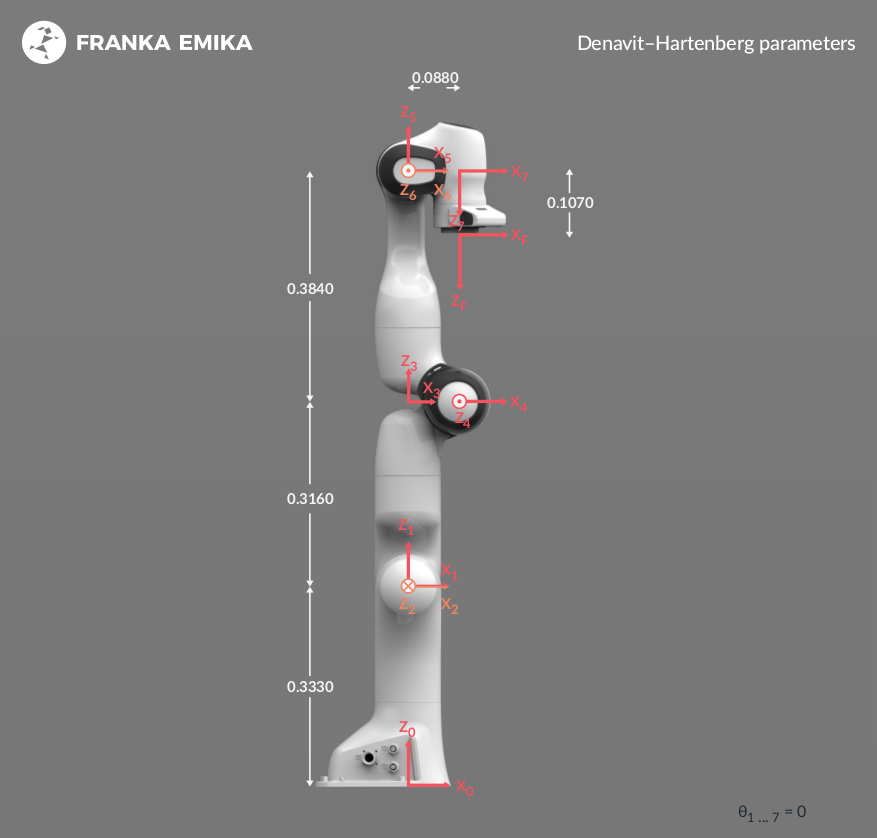
\includegraphics[max width=0.6\textwidth]{kinematics/dh-diagram.png}
    \caption{Panda’s kinematic chain}
\end{figure}


\begin{figure}[H]
    \centering
    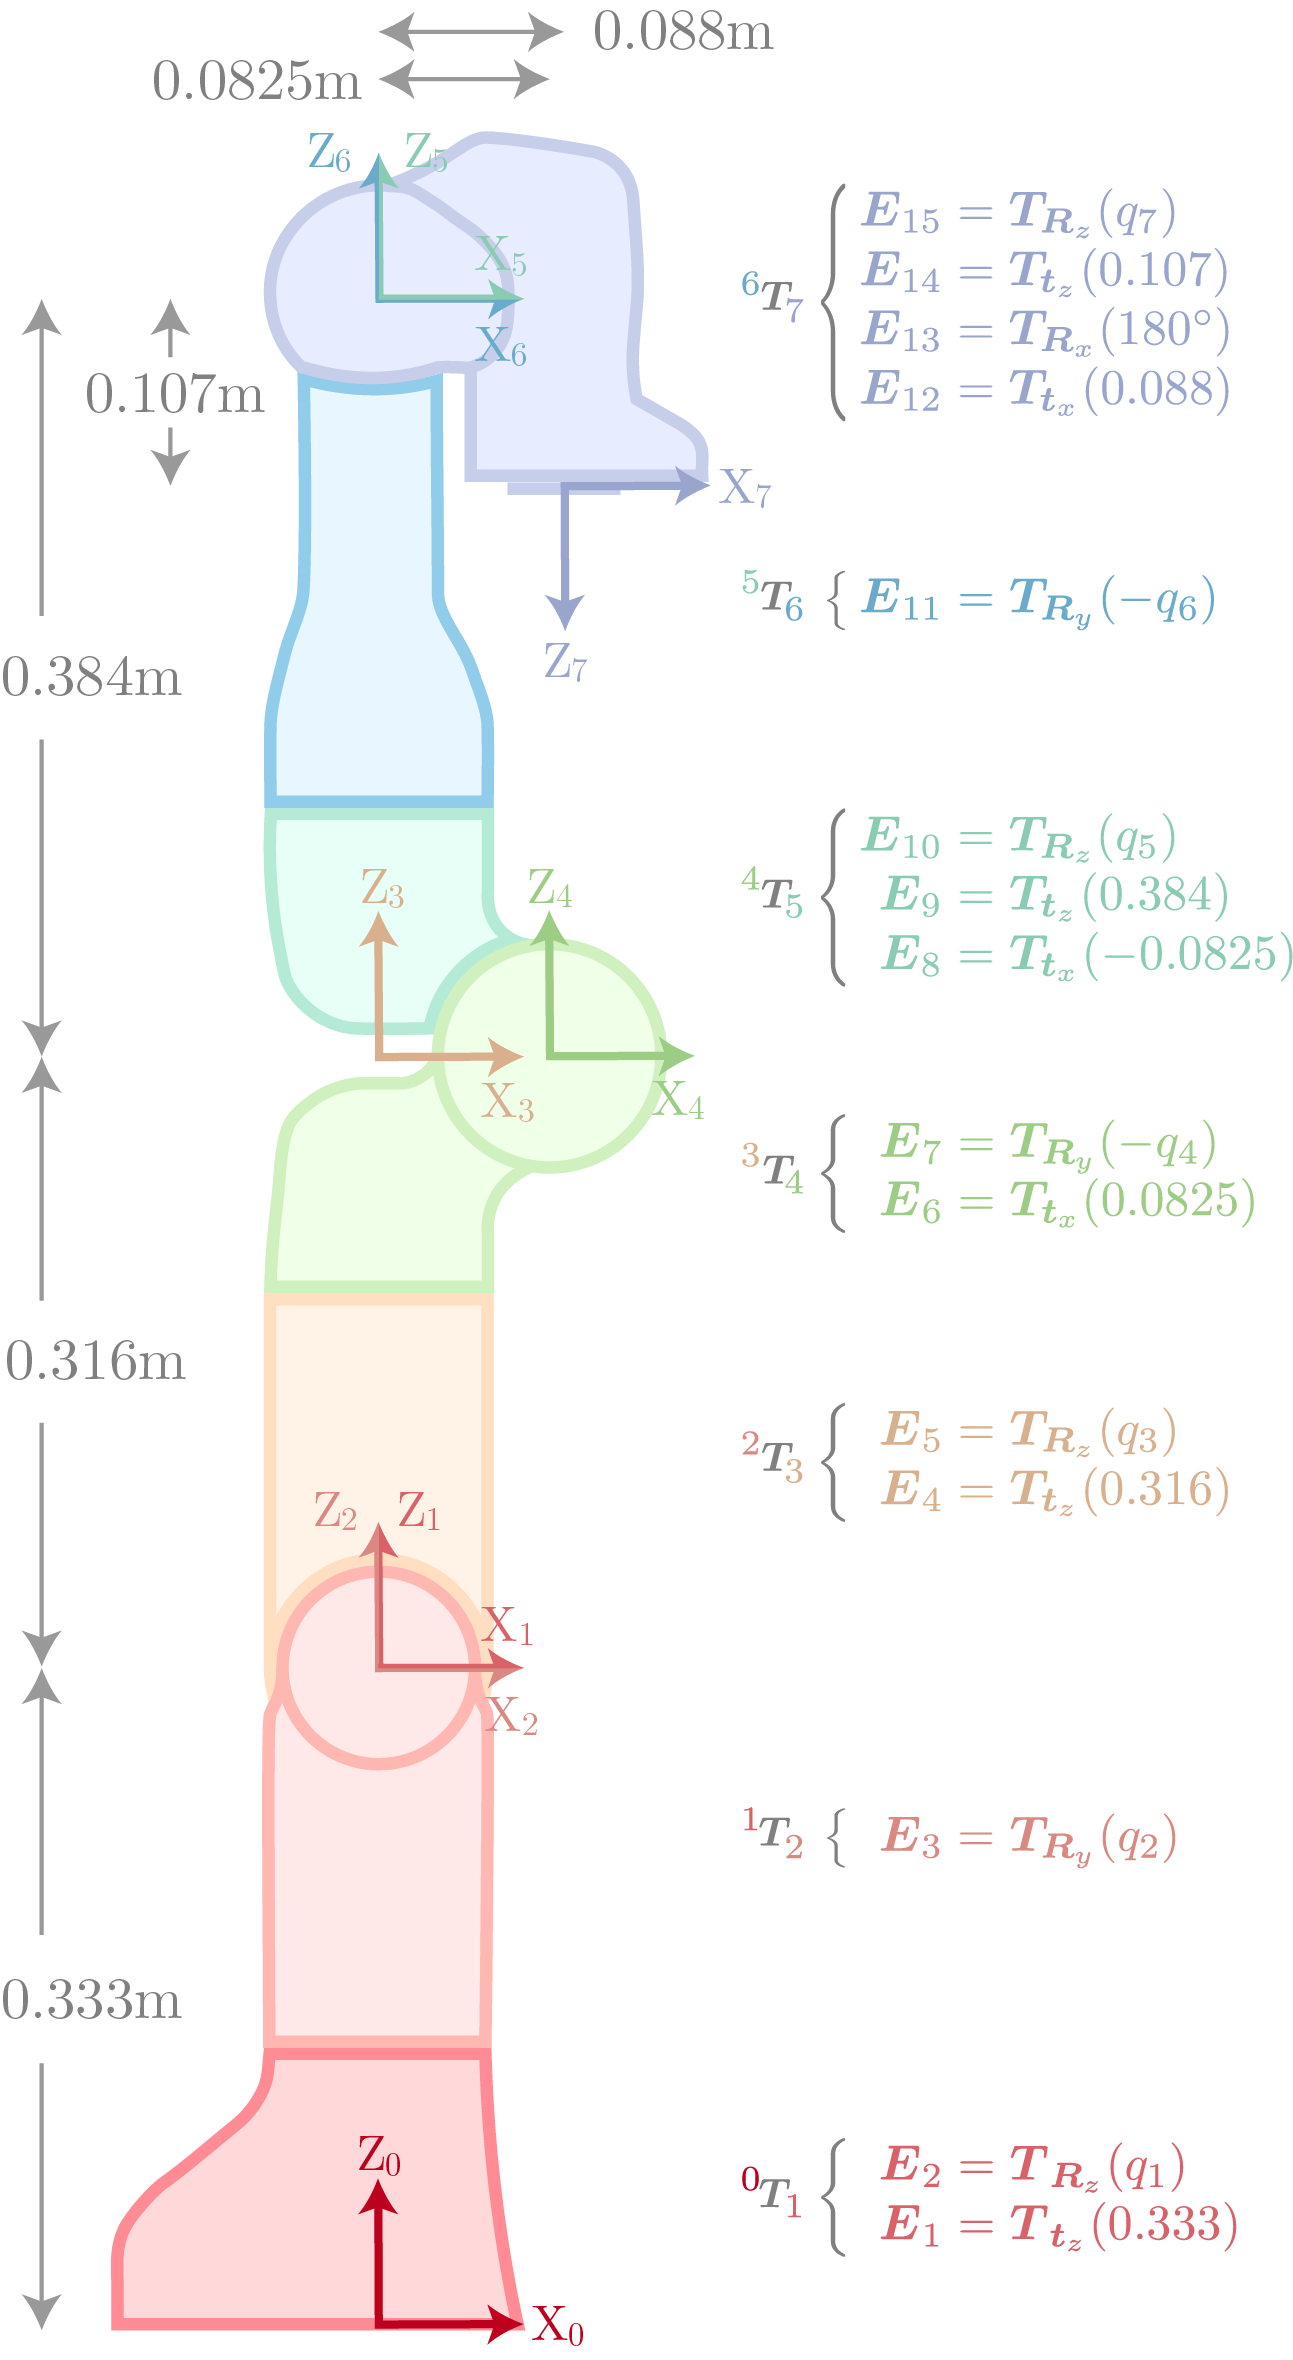
\includegraphics[max width=0.3\textwidth]{kinematics/cover.png}
    \caption{Panda’s kinematic chain (from Peter Corke's Tutorial)}
\end{figure}


\end{document}


